\begin{enumerate}
    \item  
    Khi xoay bánh răng với một tần số nhất định, ánh sáng sẽ có lúc đập vào răng, sẽ có lúc đi qua khe giữa hai răng liên tiếp. Xét trường hợp đi qua khe, khi đó ánh sáng chiếu đến gương 2 và phản xạ lại. Nếu bánh răng quay đủ chậm, ánh sáng sẽ trở lại đúng với khe đó, phản xạ với gương bán mạ và tới mặt. Nhưng nếu ta tăng dần tần số thì tại một tần số $f$, sẽ có trường hợp ánh sáng đập vào răng, khiến ta không thấy gì. Lúc này, thời gian quay từ khe tới bánh răng thứ hai sẽ chính là thời gian ánh sáng đi quãng đường $2L$. \\

    Quãng đường một bánh răng đi được trong khoảng thời gian $T$:
    \begin{equation}
        s = 2 \pi R f T.
    \end{equation}
    Suy ra vận tốc của một bánh răng:
    \begin{equation}
        v = \frac{s}{T} = 2 \pi R f.
    \end{equation}
    Trên chu vi bánh răng sẽ có $n$ bánh răng và $n$ khoảng trống giữa các bánh răng. Vì các khoảng trống này có kích thước bằng các bánh răng nên khoảng cách giữa hai bánh răng là:
    \begin{equation}
        d = \frac{2 \pi R}{2n} = \frac{\pi R}{n}.
    \end{equation}
    Suy ra thời gian đi của khe 1 đến khe 2 (hay từ A đến B, như trên hình $\ref{fig:03}$):
    \begin{equation}
        t = \frac{d}{v} = \frac{1}{2nf}.
    \end{equation}
    
    \begin{figure}[!h]
    \centering
    \scalebox{0.9}{
    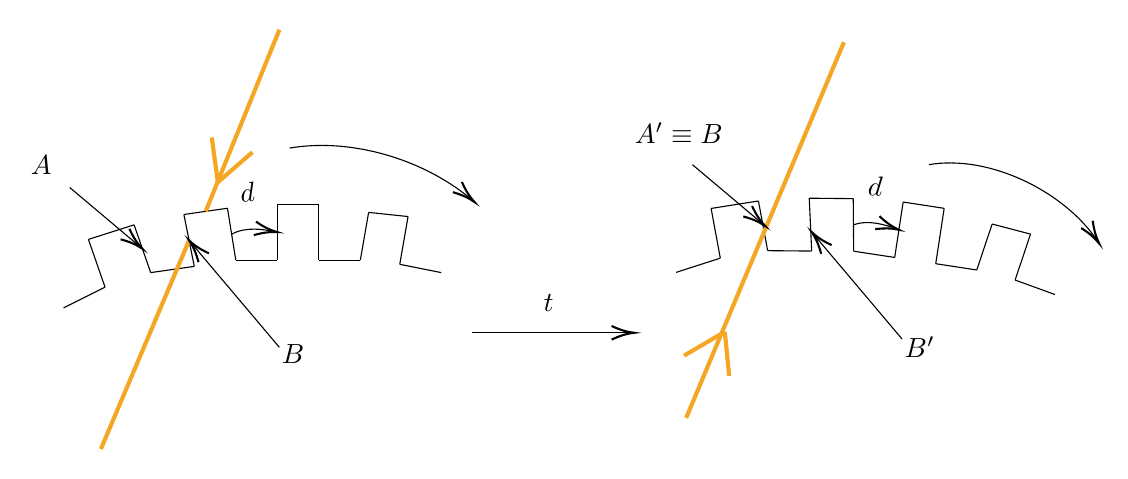
\begin{tikzpicture}[x=0.75pt,y=0.75pt,yscale=-1,xscale=1]
        %uncomment if require: \path (0,300); %set diagram left start at 0, and has height of 300
        
        %Straight Lines [id:da16583505343459715] 
        \draw    (112,164) -- (104,141) ;
        %Straight Lines [id:da1843590505275179] 
        \draw    (104,141) -- (126,134) ;
        %Straight Lines [id:da826646904856134] 
        \draw    (134,157) -- (126,134) ;
        %Straight Lines [id:da3557506388733678] 
        \draw    (155,154) -- (134,157) ;
        %Straight Lines [id:da5882845065003475] 
        \draw    (155,154) -- (150,129) ;
        %Straight Lines [id:da6729219415271026] 
        \draw    (150,129) -- (171,126) ;
        %Straight Lines [id:da5201523005778395] 
        \draw    (171,126) -- (175,151) ;
        %Straight Lines [id:da14816797362150558] 
        \draw    (195,151) -- (175,151) ;
        %Straight Lines [id:da14480513606262946] 
        \draw    (195,124) -- (195,151) ;
        %Straight Lines [id:da6227327136235512] 
        \draw    (195,124) -- (215,124) ;
        %Straight Lines [id:da34141038968741766] 
        \draw    (215,124) -- (215,151) ;
        %Straight Lines [id:da6029080535909679] 
        \draw    (235,151) -- (215,151) ;
        %Straight Lines [id:da47292252824911896] 
        \draw    (239,128) -- (235,151) ;
        %Straight Lines [id:da331432785638605] 
        \draw    (258,130) -- (239,128) ;
        %Straight Lines [id:da1565969017667539] 
        \draw    (258,130) -- (254,153) ;
        %Straight Lines [id:da9917128687641255] 
        \draw    (274,157) -- (254,153) ;
        %Curve Lines [id:da6568586220124728] 
        \draw    (173,138.5) .. controls (179.76,134.7) and (188.66,136.25) .. (193.07,137.12) ;
        \draw [shift={(195,137.5)}, rotate = 189.46] [color={rgb, 255:red, 0; green, 0; blue, 0 }  ][line width=0.75]    (10.93,-3.29) .. controls (6.95,-1.4) and (3.31,-0.3) .. (0,0) .. controls (3.31,0.3) and (6.95,1.4) .. (10.93,3.29)   ;
        %Straight Lines [id:da43992497276077436] 
        \draw    (112,164) -- (92,174) ;
        %Straight Lines [id:da4470951160432266] 
        \draw [color={rgb, 255:red, 245; green, 166; blue, 35 }  ,draw opacity=1 ][fill={rgb, 255:red, 248; green, 231; blue, 28 }  ,fill opacity=1 ][line width=1.5]    (110,242) -- (152.5,141.5) ;
        %Straight Lines [id:da057489356448303] 
        \draw [color={rgb, 255:red, 245; green, 166; blue, 35 }  ,draw opacity=1 ][fill={rgb, 255:red, 248; green, 231; blue, 28 }  ,fill opacity=1 ][line width=1.5]    (166.35,113.47) -- (163.43,91.91) ;
        %Straight Lines [id:da06473912816630212] 
        \draw [color={rgb, 255:red, 245; green, 166; blue, 35 }  ,draw opacity=1 ][fill={rgb, 255:red, 248; green, 231; blue, 28 }  ,fill opacity=1 ][line width=1.5]    (183,99) -- (166.35,113.47) ;
        %Straight Lines [id:da4647051584102313] 
        \draw [color={rgb, 255:red, 245; green, 166; blue, 35 }  ,draw opacity=1 ][fill={rgb, 255:red, 248; green, 231; blue, 28 }  ,fill opacity=1 ][line width=1.5]    (160.5,127.5) -- (196,40) ;
        
        %Straight Lines [id:da778085515777805] 
        \draw    (408.44,150.03) -- (404.01,126.09) ;
        %Straight Lines [id:da9838084515420793] 
        \draw    (404.01,126.09) -- (426.81,122.49) ;
        %Straight Lines [id:da19033527948258522] 
        \draw    (431.25,146.43) -- (426.81,122.49) ;
        %Straight Lines [id:da24366986239748667] 
        \draw    (452.46,146.63) -- (431.25,146.43) ;
        %Straight Lines [id:da3722296140959016] 
        \draw    (452.46,146.63) -- (451.29,121.16) ;
        %Straight Lines [id:da6654256337536733] 
        \draw    (451.29,121.16) -- (472.5,121.37) ;
        %Straight Lines [id:da5624868250097093] 
        \draw    (472.5,121.37) -- (472.68,146.69) ;
        %Straight Lines [id:da13456201918016286] 
        \draw    (492.46,149.7) -- (472.68,146.69) ;
        %Straight Lines [id:da7839463228545538] 
        \draw    (496.53,123.01) -- (492.46,149.7) ;
        %Straight Lines [id:da021076194780720536] 
        \draw    (496.53,123.01) -- (516.3,126.03) ;
        %Straight Lines [id:da2809340405486218] 
        \draw    (516.3,126.03) -- (512.23,152.72) ;
        %Straight Lines [id:da8162562337101826] 
        \draw    (532,155.74) -- (512.23,152.72) ;
        %Straight Lines [id:da5508701922826711] 
        \draw    (539.42,133.61) -- (532,155.74) ;
        %Straight Lines [id:da2073569786271683] 
        \draw    (557.9,138.45) -- (539.42,133.61) ;
        %Straight Lines [id:da05281766764100504] 
        \draw    (557.9,138.45) -- (550.48,160.59) ;
        %Straight Lines [id:da9267167847965421] 
        \draw    (569.65,167.56) -- (550.48,160.59) ;
        %Curve Lines [id:da25941570234382905] 
        \draw    (472.59,134.03) .. controls (479.85,131.29) and (488.42,134.17) .. (492.64,135.7) ;
        \draw [shift={(494.49,136.36)}, rotate = 198.14] [color={rgb, 255:red, 0; green, 0; blue, 0 }  ][line width=0.75]    (10.93,-3.29) .. controls (6.95,-1.4) and (3.31,-0.3) .. (0,0) .. controls (3.31,0.3) and (6.95,1.4) .. (10.93,3.29)   ;
        %Straight Lines [id:da25719999452816844] 
        \draw    (408.44,150.03) -- (387.16,156.9) ;
        
        %Straight Lines [id:da9866819779007816] 
        \draw [color={rgb, 255:red, 245; green, 166; blue, 35 }  ,draw opacity=1 ][fill={rgb, 255:red, 248; green, 231; blue, 28 }  ,fill opacity=1 ][line width=1.5]    (392,227) -- (420.3,159.38) -- (468,46) ;
        %Straight Lines [id:da8907940513806709] 
        \draw [color={rgb, 255:red, 245; green, 166; blue, 35 }  ,draw opacity=1 ][fill={rgb, 255:red, 248; green, 231; blue, 28 }  ,fill opacity=1 ][line width=1.5]    (410.61,185.51) -- (412.73,206.87) ;
        %Straight Lines [id:da6856666463935532] 
        \draw [color={rgb, 255:red, 245; green, 166; blue, 35 }  ,draw opacity=1 ][fill={rgb, 255:red, 248; green, 231; blue, 28 }  ,fill opacity=1 ][line width=1.5]    (391,197) -- (410.61,185.51) ;
        
        %Straight Lines [id:da5029343983238321] 
        \draw    (289,186) -- (365,186) ;
        \draw [shift={(367,186)}, rotate = 180] [color={rgb, 255:red, 0; green, 0; blue, 0 }  ][line width=0.75]    (10.93,-3.29) .. controls (6.95,-1.4) and (3.31,-0.3) .. (0,0) .. controls (3.31,0.3) and (6.95,1.4) .. (10.93,3.29)   ;
        %Straight Lines [id:da5945341647364351] 
        \draw    (95,116) -- (128.47,144.21) ;
        \draw [shift={(130,145.5)}, rotate = 220.13] [color={rgb, 255:red, 0; green, 0; blue, 0 }  ][line width=0.75]    (10.93,-3.29) .. controls (6.95,-1.4) and (3.31,-0.3) .. (0,0) .. controls (3.31,0.3) and (6.95,1.4) .. (10.93,3.29)   ;
        %Straight Lines [id:da8901129955737317] 
        \draw    (196,193) -- (153.79,143.03) ;
        \draw [shift={(152.5,141.5)}, rotate = 49.81] [color={rgb, 255:red, 0; green, 0; blue, 0 }  ][line width=0.75]    (10.93,-3.29) .. controls (6.95,-1.4) and (3.31,-0.3) .. (0,0) .. controls (3.31,0.3) and (6.95,1.4) .. (10.93,3.29)   ;
        %Straight Lines [id:da5860393867941966] 
        \draw    (395,105) -- (428.47,133.21) ;
        \draw [shift={(430,134.5)}, rotate = 220.13] [color={rgb, 255:red, 0; green, 0; blue, 0 }  ][line width=0.75]    (10.93,-3.29) .. controls (6.95,-1.4) and (3.31,-0.3) .. (0,0) .. controls (3.31,0.3) and (6.95,1.4) .. (10.93,3.29)   ;
        %Straight Lines [id:da4406388844428304] 
        \draw    (496,189) -- (453.79,139.03) ;
        \draw [shift={(452.5,137.5)}, rotate = 49.81] [color={rgb, 255:red, 0; green, 0; blue, 0 }  ][line width=0.75]    (10.93,-3.29) .. controls (6.95,-1.4) and (3.31,-0.3) .. (0,0) .. controls (3.31,0.3) and (6.95,1.4) .. (10.93,3.29)   ;
        %Curve Lines [id:da1863112199988879] 
        \draw    (201,97) .. controls (229.42,92.1) and (264.56,101.61) .. (288.55,121.75) ;
        \draw [shift={(290,123)}, rotate = 221.19] [color={rgb, 255:red, 0; green, 0; blue, 0 }  ][line width=0.75]    (10.93,-3.29) .. controls (6.95,-1.4) and (3.31,-0.3) .. (0,0) .. controls (3.31,0.3) and (6.95,1.4) .. (10.93,3.29)   ;
        %Curve Lines [id:da8552192716449836] 
        \draw    (509,105) .. controls (537.42,100.1) and (573.52,117.29) .. (590.02,141.51) ;
        \draw [shift={(591,143)}, rotate = 237.38] [color={rgb, 255:red, 0; green, 0; blue, 0 }  ][line width=0.75]    (10.93,-3.29) .. controls (6.95,-1.4) and (3.31,-0.3) .. (0,0) .. controls (3.31,0.3) and (6.95,1.4) .. (10.93,3.29)   ;
        
        % Text Node
        \draw (478.69,109.19) node [anchor=north west][inner sep=0.75pt]  [rotate=-3.02]  {$d$};
        % Text Node
        \draw (322,166.4) node [anchor=north west][inner sep=0.75pt]    {$t$};
        % Text Node
        \draw (75,99.4) node [anchor=north west][inner sep=0.75pt]    {$A$};
        % Text Node
        \draw (196,190.4) node [anchor=north west][inner sep=0.75pt]    {$B$};
        % Text Node
        \draw (175.28,113.03) node [anchor=north west][inner sep=0.75pt]  [rotate=-354.34]  {$d$};
        % Text Node
        \draw (366,83.4) node [anchor=north west][inner sep=0.75pt]    {$A'\equiv B$};
        % Text Node
        \draw (496,186.4) node [anchor=north west][inner sep=0.75pt]    {$B'$};
        
        
    \end{tikzpicture}
    }
    
    \caption{Hình ảnh di chuyển của răng bánh}
    \label{fig:03}
\end{figure}

    Thời gian ánh sáng từ B, chạm vào gương $G_2$ và sau đó đi qua A':
    \begin{equation}
        t_S = \frac{2L}{c}.
    \end{equation}
    Vì thời gian ánh sáng đi một quãng đường dài $2L$ bằng với thời gian bánh răng đi từ vị trí $A$ đến vị trí $B$ như trên Hình $\ref{fig:03}$ nên ta có:
    \begin{equation}
        \frac{1}{2nf} = \frac{2L}{c} \Rightarrow c = 4Lnf.
        \label{eq:01}
    \end{equation}

    \item 
    Thay số vào (\ref{eq:01}), ta được:
    \begin{equation}
        c = 4 \times 8630 \times 720 \times 12.6 = \SI{313 000 000}{m/s}.
    \end{equation}
    Phần trăm chênh lệch so với giá trị hiện nay:
    \begin{equation}
        \Delta c = \frac{313 000 000 - 299 792 458}{299 792 458} \times 100 \% \simeq 4.41 \%.
    \end{equation}
    Vậy vận tốc mà Fizeau đo cao hơn $4.41\%$ so với giá trị chính xác hiện nay.
    
    \item 
    Nếu không khởi động motor, gương $G_4$ không xoay thì đường truyền của tia sáng sẽ là $(a) \xrightarrow{G_4} (b) \xrightarrow{G_5} (b) \xrightarrow{G_4} (a) \xrightarrow{G_3} E_1$. \\
    
    Nếu motor khởi động, gương $G_4$ bắt đầu xoay thì đường truyền tia sáng sẽ là $(a) \xrightarrow{G_4} (b) \xrightarrow{G_5} (b) \xrightarrow{G_4} (c) \xrightarrow{G_3} E_2$. \\
    
    Khi này, dựa vào độ thay đổi của góc $\Delta \theta$ và độ thay đổi của tia sáng trên tấm kính mờ $\Delta x$, ta có thể dùng các kiến thức hình học và lượng giác để xác định vận tốc ánh sáng. \\

    Gọi $\tau$ là thời gian ánh sáng từ guơng $G_4$ đi tới gương $G_5$, sau khi phản xạ thì quay về lại $G_4$. Ta có:
    \begin{equation}
        \tau = \frac{2D}{c}.
        \label{eq:02}
    \end{equation}
    Trong 1 giây thì gương xoay được $f$ vòng, tức một điểm trên gương sẽ xoay được một góc $2 \pi f$ quanh tâm của gương. Ta định nghĩa \textbf{vận tốc góc} $\omega$:
    \begin{equation}
        \omega = \frac{\Delta \alpha}{\Delta t} = 2 \pi f.
    \end{equation}
    là độ biến thiên góc $\Delta \alpha$ của một điểm chuyển động tròn đều quanh một tâm xác định trong khoảng thời gian $\Delta t$. Giả sử trong thời gian $\tau$ gương quay được một góc $\Delta \theta$, ta sẽ có:
    \begin{equation}
        \tau = \frac{\Delta \theta}{\omega} = \frac{\Delta \theta}{2 \pi f}.
        \label{eq:03}
    \end{equation}
    Khi gương $G_4$ quay được một góc $\Delta\theta$ thì góc tạo bởi tia sáng $(a)$ và $(c)$ sẽ là $2 \Delta\theta$. Vì góc $2 \Delta\theta$ rất nhỏ nên ta có thể xấp xỉ $\tan(2 \Delta\theta) \approx 2 \Delta\theta$ như đã cung cấp ở đề bài. Từ điều này, ta sẽ xấp xỉ những giá trị khác như trong Hình $\ref{fig:04}$, sao cho thuận tiện trong tính toán nhất có thể. Từ những xấp xỉ trên, ta có:

    \begin{figure}[!h]
    \centering
    \scalebox{0.9}{
    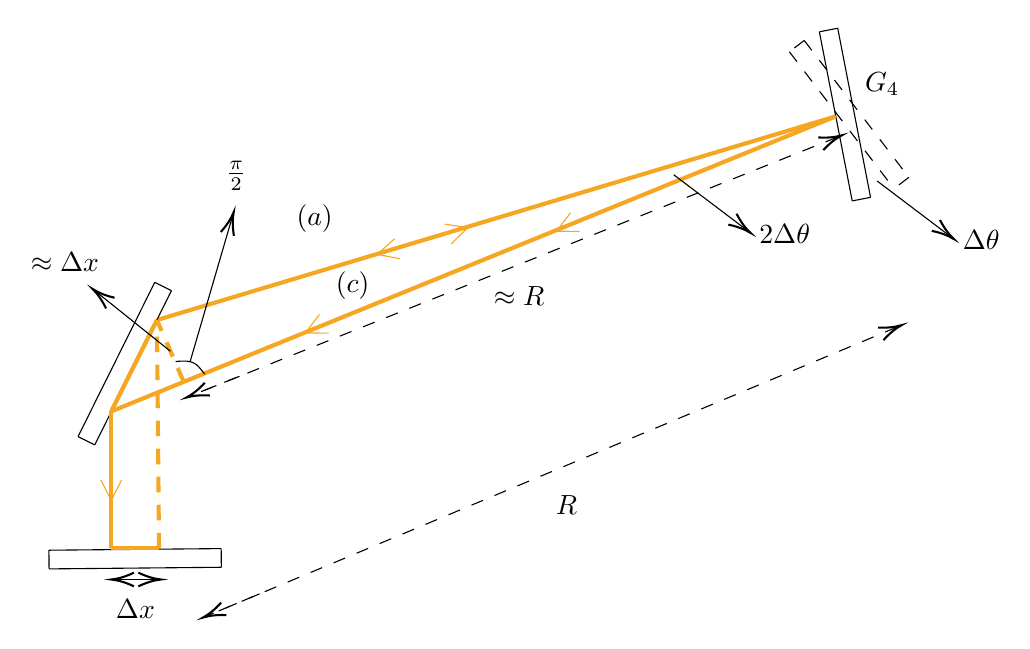
\begin{tikzpicture}[x=0.75pt,y=0.75pt,yscale=-1,xscale=1]
    %uncomment if require: \path (0,376); %set diagram left start at 0, and has height of 376
    
    %Straight Lines [id:da43129234255320026] 
    \draw [color={rgb, 255:red, 245; green, 166; blue, 35 }  ,draw opacity=1 ][fill={rgb, 255:red, 248; green, 231; blue, 28 }  ,fill opacity=1 ][line width=1.5]    (175,172) -- (502.08,73.86) ;
    %Straight Lines [id:da07771062362227799] 
    \draw    (494.17,33.12) -- (509.99,114.6) ;
    %Straight Lines [id:da278105123364655] 
    \draw    (503.01,31.4) -- (518.83,112.88) ;
    %Straight Lines [id:da9235969449614554] 
    \draw    (503.01,31.4) -- (494.17,33.12) ;
    %Straight Lines [id:da2894919968044616] 
    \draw    (518.83,112.88) -- (509.99,114.6) ;
    
    \draw  [color={rgb, 255:red, 245; green, 166; blue, 35 }  ,draw opacity=1 ] (313.69,125.81) -- (324.75,127.44) -- (316.81,135.31) ;
    %Straight Lines [id:da06778307505143855] 
    \draw  [dash pattern={on 4.5pt off 4.5pt}]  (479.73,42.75) -- (530.12,108.71) ;
    %Straight Lines [id:da9966267511565405] 
    \draw  [dash pattern={on 4.5pt off 4.5pt}]  (486.88,37.29) -- (537.27,103.25) ;
    %Straight Lines [id:da9100321561845419] 
    \draw  [dash pattern={on 4.5pt off 4.5pt}]  (486.88,37.29) -- (479.73,42.75) ;
    
    %Straight Lines [id:da36191204723490267] 
    \draw  [dash pattern={on 4.5pt off 4.5pt}]  (537.27,103.25) -- (530.12,108.71) ;
    
    %Straight Lines [id:da1329383626996341] 
    \draw    (173.96,153.84) -- (136.99,228.15) ;
    %Straight Lines [id:da4110555525593613] 
    \draw    (182.01,157.85) -- (145.04,232.16) ;
    %Straight Lines [id:da3392299552891971] 
    \draw    (182.01,157.85) -- (173.96,153.84) ;
    %Straight Lines [id:da7708519672664513] 
    \draw    (145.04,232.16) -- (136.99,228.15) ;
    
    %Straight Lines [id:da6443951388175031] 
    \draw [color={rgb, 255:red, 245; green, 166; blue, 35 }  ,draw opacity=1 ][fill={rgb, 255:red, 248; green, 231; blue, 28 }  ,fill opacity=1 ][line width=1.5]    (153,216) -- (502.08,73.86) ;
    %Straight Lines [id:da014449999702887517] 
    \draw [color={rgb, 255:red, 245; green, 166; blue, 35 }  ,draw opacity=1 ][fill={rgb, 255:red, 248; green, 231; blue, 28 }  ,fill opacity=1 ][line width=1.5]  [dash pattern={on 5.63pt off 4.5pt}]  (176,282) -- (175,172) ;
    %Straight Lines [id:da17097694263904417] 
    \draw [color={rgb, 255:red, 245; green, 166; blue, 35 }  ,draw opacity=1 ][fill={rgb, 255:red, 248; green, 231; blue, 28 }  ,fill opacity=1 ][line width=1.5]    (153,282) -- (153,216) ;
    %Straight Lines [id:da9782141464033616] 
    \draw    (205.96,282.11) -- (122.96,282.89) ;
    %Straight Lines [id:da6111393813376975] 
    \draw    (206.04,291.11) -- (123.04,291.89) ;
    %Straight Lines [id:da9391806826198021] 
    \draw    (206.04,291.11) -- (205.96,282.11) ;
    %Straight Lines [id:da22726742466966843] 
    \draw    (123.04,291.89) -- (122.96,282.89) ;
    
    %Straight Lines [id:da9162627871348716] 
    \draw  [dash pattern={on 4.5pt off 4.5pt}]  (204.8,312.14) -- (532.01,175.2) ;
    \draw [shift={(533.85,174.43)}, rotate = 157.29] [color={rgb, 255:red, 0; green, 0; blue, 0 }  ][line width=0.75]    (10.93,-3.29) .. controls (6.95,-1.4) and (3.31,-0.3) .. (0,0) .. controls (3.31,0.3) and (6.95,1.4) .. (10.93,3.29)   ;
    %Straight Lines [id:da2895911805275999] 
    \draw  [dash pattern={on 4.5pt off 4.5pt}]  (224.48,303.91) -- (198.99,314.58) ;
    \draw [shift={(197.15,315.35)}, rotate = 337.29] [color={rgb, 255:red, 0; green, 0; blue, 0 }  ][line width=0.75]    (10.93,-3.29) .. controls (6.95,-1.4) and (3.31,-0.3) .. (0,0) .. controls (3.31,0.3) and (6.95,1.4) .. (10.93,3.29)   ;
    
    %Straight Lines [id:da3411787710606038] 
    \draw    (153,297) -- (175,297) ;
    \draw [shift={(177,297)}, rotate = 180] [color={rgb, 255:red, 0; green, 0; blue, 0 }  ][line width=0.75]    (10.93,-3.29) .. controls (6.95,-1.4) and (3.31,-0.3) .. (0,0) .. controls (3.31,0.3) and (6.95,1.4) .. (10.93,3.29)   ;
    %Straight Lines [id:da6326235218553786] 
    \draw    (165,297) -- (155,297) ;
    \draw [shift={(153,297)}, rotate = 360] [color={rgb, 255:red, 0; green, 0; blue, 0 }  ][line width=0.75]    (10.93,-3.29) .. controls (6.95,-1.4) and (3.31,-0.3) .. (0,0) .. controls (3.31,0.3) and (6.95,1.4) .. (10.93,3.29)   ;
    %Straight Lines [id:da8744107678030113] 
    \draw    (522,105) -- (557.41,131.79) ;
    \draw [shift={(559,133)}, rotate = 217.12] [color={rgb, 255:red, 0; green, 0; blue, 0 }  ][line width=0.75]    (10.93,-3.29) .. controls (6.95,-1.4) and (3.31,-0.3) .. (0,0) .. controls (3.31,0.3) and (6.95,1.4) .. (10.93,3.29)   ;
    \draw  [color={rgb, 255:red, 245; green, 166; blue, 35 }  ,draw opacity=1 ] (378.68,129.31) -- (367.5,129.19) -- (374.31,120.32) ;
    \draw  [color={rgb, 255:red, 245; green, 166; blue, 35 }  ,draw opacity=1 ] (257.68,178.31) -- (246.5,178.19) -- (253.31,169.32) ;
    \draw  [color={rgb, 255:red, 245; green, 166; blue, 35 }  ,draw opacity=1 ] (292.15,142.5) -- (281.18,140.33) -- (289.5,132.85) ;
    \draw  [color={rgb, 255:red, 245; green, 166; blue, 35 }  ,draw opacity=1 ] (157.99,248.99) -- (153.01,259) -- (147.99,249.01) ;
    %Straight Lines [id:da5674171617561174] 
    \draw [color={rgb, 255:red, 245; green, 166; blue, 35 }  ,draw opacity=1 ][fill={rgb, 255:red, 248; green, 231; blue, 28 }  ,fill opacity=1 ][line width=1.5]    (153,216) -- (175,172) ;
    %Straight Lines [id:da4980966569900862] 
    \draw [color={rgb, 255:red, 245; green, 166; blue, 35 }  ,draw opacity=1 ][fill={rgb, 255:red, 248; green, 231; blue, 28 }  ,fill opacity=1 ][line width=1.5]    (153,282) -- (176,282) ;
    %Straight Lines [id:da4667494460114985] 
    \draw    (424,102) -- (459.41,128.79) ;
    \draw [shift={(461,130)}, rotate = 217.12] [color={rgb, 255:red, 0; green, 0; blue, 0 }  ][line width=0.75]    (10.93,-3.29) .. controls (6.95,-1.4) and (3.31,-0.3) .. (0,0) .. controls (3.31,0.3) and (6.95,1.4) .. (10.93,3.29)   ;
    %Straight Lines [id:da28230446932613784] 
    \draw    (191,192) -- (211.44,121.92) ;
    \draw [shift={(212,120)}, rotate = 106.26] [color={rgb, 255:red, 0; green, 0; blue, 0 }  ][line width=0.75]    (10.93,-3.29) .. controls (6.95,-1.4) and (3.31,-0.3) .. (0,0) .. controls (3.31,0.3) and (6.95,1.4) .. (10.93,3.29)   ;
    %Curve Lines [id:da35850377354211505] 
    \draw    (184,192) .. controls (193,191) and (194,193) .. (198,198) ;
    %Straight Lines [id:da22083259694217472] 
    \draw [color={rgb, 255:red, 245; green, 166; blue, 35 }  ,draw opacity=1 ][fill={rgb, 255:red, 248; green, 231; blue, 28 }  ,fill opacity=1 ][line width=1.5]  [dash pattern={on 5.63pt off 4.5pt}]  (188,202) -- (175,172) ;
    %Straight Lines [id:da7767254708982354] 
    \draw    (181.5,187) -- (145.56,158.25) ;
    \draw [shift={(144,157)}, rotate = 38.66] [color={rgb, 255:red, 0; green, 0; blue, 0 }  ][line width=0.75]    (10.93,-3.29) .. controls (6.95,-1.4) and (3.31,-0.3) .. (0,0) .. controls (3.31,0.3) and (6.95,1.4) .. (10.93,3.29)   ;
    %Straight Lines [id:da410010118198592] 
    \draw  [dash pattern={on 4.5pt off 4.5pt}]  (196.33,206.48) -- (503.14,83.74) ;
    \draw [shift={(505,83)}, rotate = 158.2] [color={rgb, 255:red, 0; green, 0; blue, 0 }  ][line width=0.75]    (10.93,-3.29) .. controls (6.95,-1.4) and (3.31,-0.3) .. (0,0) .. controls (3.31,0.3) and (6.95,1.4) .. (10.93,3.29)   ;
    %Straight Lines [id:da5885427911439025] 
    \draw  [dash pattern={on 4.5pt off 4.5pt}]  (214.79,199.09) -- (191.01,208.6) ;
    \draw [shift={(189.15,209.35)}, rotate = 338.2] [color={rgb, 255:red, 0; green, 0; blue, 0 }  ][line width=0.75]    (10.93,-3.29) .. controls (6.95,-1.4) and (3.31,-0.3) .. (0,0) .. controls (3.31,0.3) and (6.95,1.4) .. (10.93,3.29)   ;
    
    
    % Text Node
    \draw (366,255.4) node [anchor=north west][inner sep=0.75pt]    {$R$};
    % Text Node
    \draw (154,305.4) node [anchor=north west][inner sep=0.75pt]    {$\Delta x$};
    % Text Node
    \draw (515,51.4) node [anchor=north west][inner sep=0.75pt]    {$G_{4}$};
    % Text Node
    \draw (562,127.4) node [anchor=north west][inner sep=0.75pt]    {$\Delta \theta $};
    % Text Node
    \draw (241,115.4) node [anchor=north west][inner sep=0.75pt]    {$( a)$};
    % Text Node
    \draw (260,147.4) node [anchor=north west][inner sep=0.75pt]    {$( c)$};
    % Text Node
    \draw (113,138.4) node [anchor=north west][inner sep=0.75pt]    {$\approx \Delta x$};
    % Text Node
    \draw (464,124.4) node [anchor=north west][inner sep=0.75pt]    {$2\Delta \theta $};
    % Text Node
    \draw (207,94.4) node [anchor=north west][inner sep=0.75pt]    {$ \frac{\pi }{2}$};
    % Text Node
    \draw (336.14,154.81) node [anchor=north west][inner sep=0.75pt]    {$\approx R$};
    
    
    \end{tikzpicture}
         }
    \caption{Các phép xấp xỉ}
    \label{fig:04}
\end{figure}

    \begin{equation}
        \tan(2 \Delta \theta) \approx 2 \Delta \theta \approx \frac{\Delta x}{R}.
        \label{eq:04}
    \end{equation}

    Thay $\Delta \theta$ từ (\ref{eq:04}) và $\tau$ từ (\ref{eq:02}) vào phương trình (\ref{eq:03}), ta được:
    
    \begin{equation}
        \frac{2D}{c} = \frac{\Delta x }{4 \pi Rf} \Rightarrow c = \frac{8 \pi D R f}{\Delta x}.
        \label{eq:05}
    \end{equation}

    \item 
    Phần trăm chênh lệch so với giá trị hiện nay:
    \begin{equation}
        \Delta c = \frac{298 000 000 - 299 792 458}{299 792 458} \times 100 \% \simeq -0.6 \%.
    \end{equation}
    Vậy vận tốc mà Foucault đo nhỏ hơn $0.6\%$ so với giá trị chính xác hiện nay. So với phần trăm chênh lệch của thí nghiệm của Fizeau ($4.41 \%$) thì thí nghiệm của Foucault hiệu quả hơn.
    
    \item \textbf{Phổ điểm}
    
    \begin{center}
    \begin{tabular}{|c|p{8cm}|c|}
    \hline
    \multicolumn{1}{|l|}{Phần} & Nội dung & Điểm thành phần \\ 
    \hline
    \multirow{3}{*}{1}
    & Xác định vận tốc của một bánh răng & 0.25 \\
    \cline{2-3} 
    & Xác định khoảng cách giữa hai bánh răng & 0.25 \\
    \cline{2-3} 
    & Thiết lập công thức tính vận tốc ánh sáng & 0.5 \\
    \hline
    2 & Thay số vào và tính đúng & 0.25 \\
    \hline
    \multirow{5}{*}{3}         
    & Thiết lập phương trình $(\ref{eq:02})$ & 0.25 \\
    \cline{2-3} 
    & Xác định được công thức liên hệ giữa thời gian gương quay và góc quay của gương & 0.50 \\
    \cline{2-3} 
    & Lập luận góc tạo bởi hai tia $(a)$ và $(c)$ là $2 \Delta \theta$ & 0.25 \\
    \cline{2-3}
    & Lấy được các phép xấp xỉ trong hình $\ref{fig:04}$ và phép xấp xỉ trong phương trình $(\ref{eq:04})$ & 1.00 (0.25 cho mỗi phép xấp xỉ)  \\
    \cline{2-3}
    & Rút ra được phương trình $(\ref{eq:05})$ và thiết lập công thức tính vận tốc ánh sáng  & 0.50 \\
    \hline
    4 & Thay số vào và tính đúng & 0.25 \\
    \hline
    \end{tabular}
    \end{center}
    
\end{enumerate}
